For the purpose of this thesis a \textit{tensor} $\bm{T}$ \textit{of rank} $n$ is an $n$-dimensional array of complex numbers
\begin{equation}
	\bm{T} \in \mathbb{C}^{\chi_1\times\chi_2\times\dots\times\chi_n}, \quad \chi_i \in \{1, 2, \dots\}
\end{equation}
with entries
\begin{equation}
	T_{i_1i_2\dots i_n} \in \mathbb{C}, \quad i_j \in \{1, 2, \dots, \chi_j\}.
\end{equation}
\begin{figure}
	\centering
	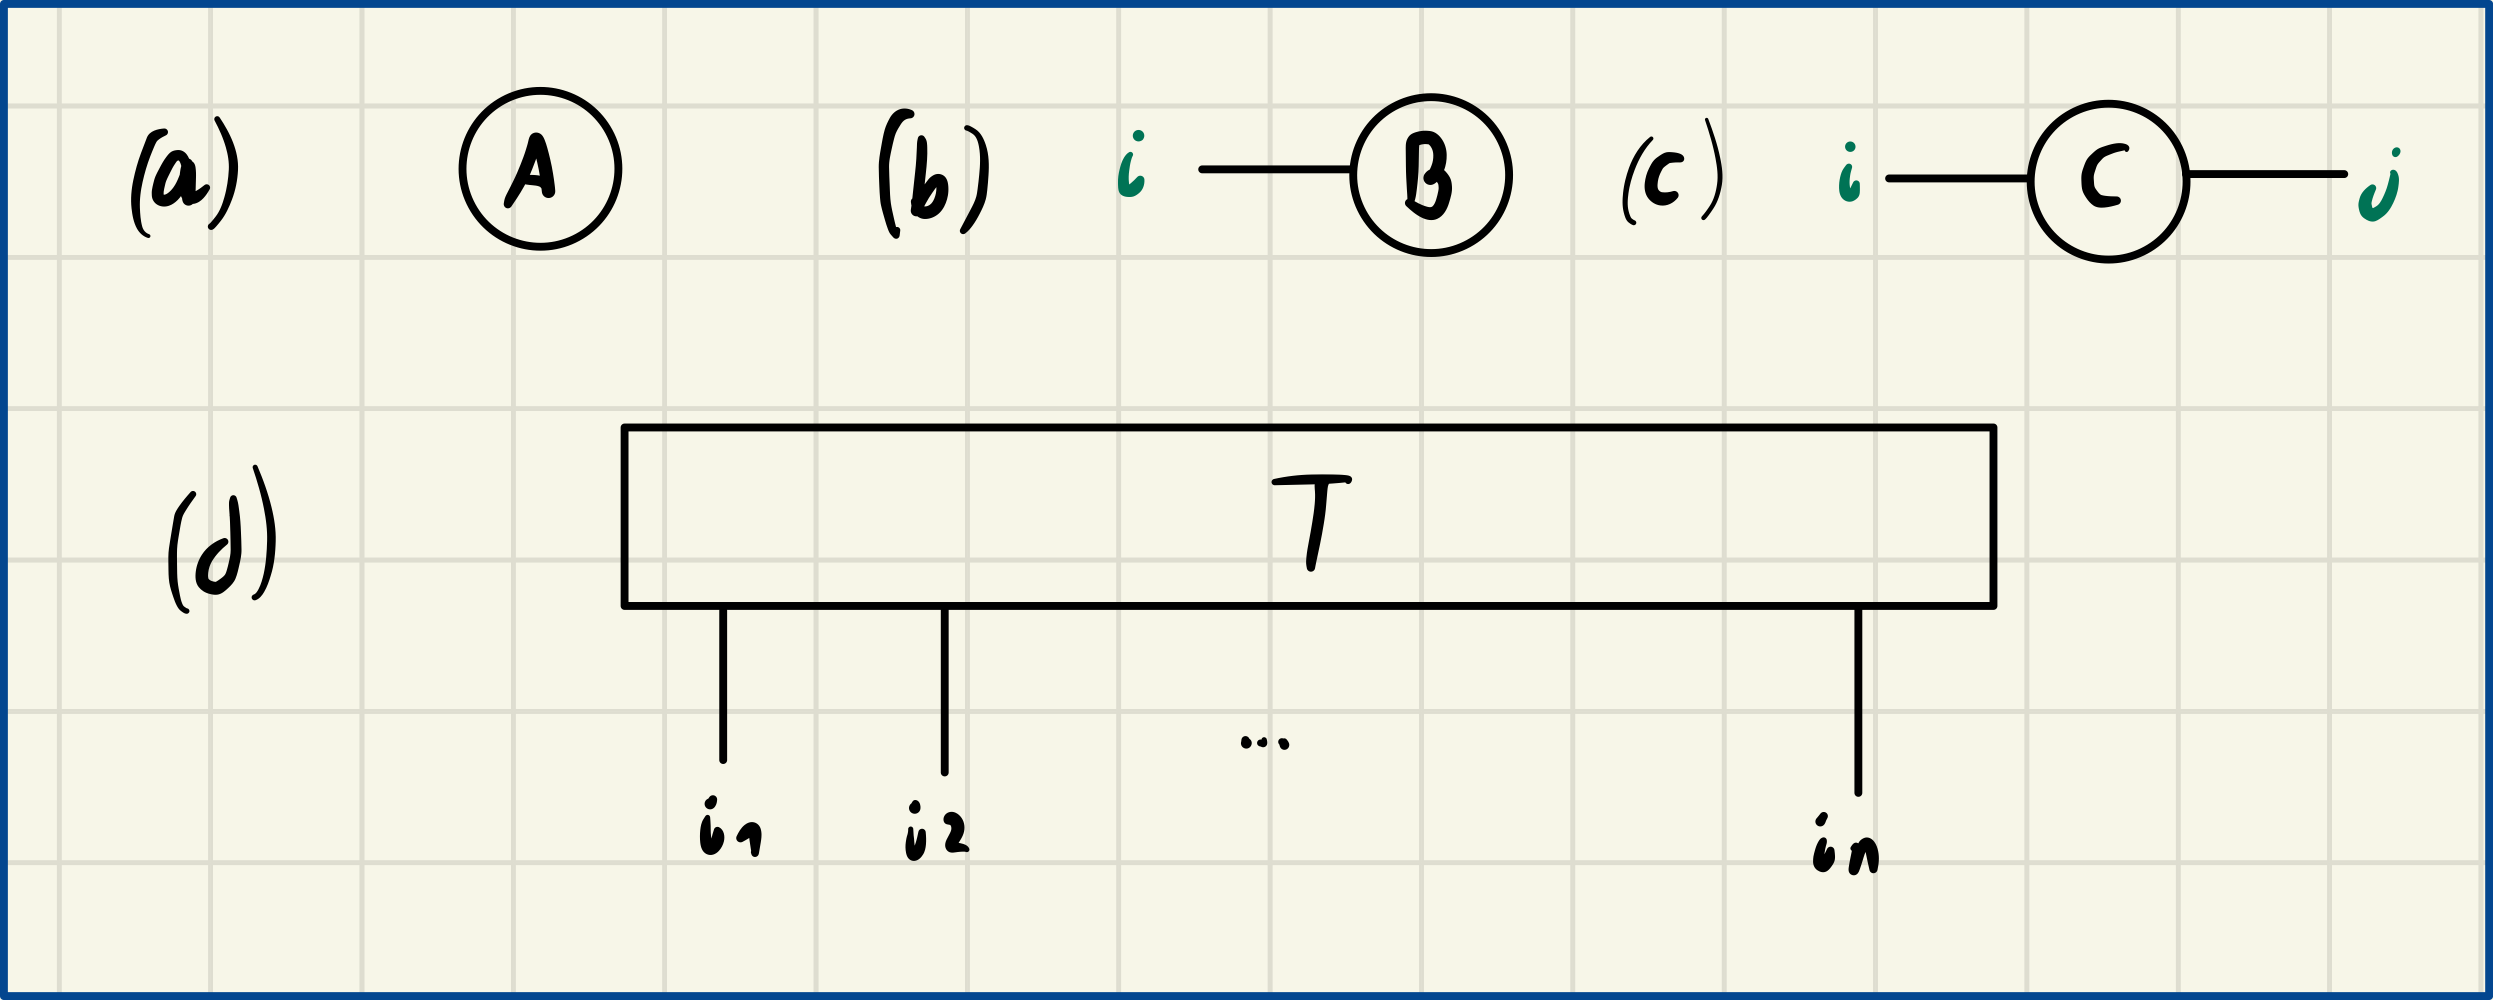
\includegraphics[width=0.8\textwidth]{figures/Tensor_Networks/basic_tensor_diagrams.jpeg}
	\caption{Tensors of different ranks are shown in diagrammatic notation. (a) A scalar $a\in\mathbb{C}$. (b) A vector $\bm{b}\in\mathbb{C}^{\chi}$. (c) A matrix $\bm{C}\in\mathbb{C}^{\chi_1\times\chi_2}$. (d) A rank-$n$ tensor $\bm{T}\in\mathbb{C}^{\chi_1\times\chi_2\times\dots\times\chi_n}$}.
	\label{fig:basic_tensor_diagrams}
\end{figure}
With this definition, a rank-0 tensor is a scalar, a rank-1 tensor is a vector, and a rank-2 tensor is a matrix. It is convenient to introduce a diagrammatic notation, where tensors are drawn as shapes and tensor indices are drawn as lines (\textit{legs}, \textit{bonds}) emerging from the shapes. To relate this diagrammatic notation to equations, one often decorates each line with the corresponding index $i_j$. A scalar, vector, matrix, and a general rank-$n$ tensor are visualized in this notation in figure \figref{fig:basic_tensor_diagrams}.\par
A \textit{tensor contraction} between two tensors along one or multiple indices is the linear operation that is given by summing over all contracted indices. Given a rank-$(n+f)$ tensor $\bm{X} \in \mathbb{C}^{\chi_1\times\dots\times\chi_n\times\xi_{1}\times\dots\times\xi_{f}}$ and a rank-$(m+f)$ tensor $\bm{Y} \in \mathbb{C}^{\lambda_1\times\dots\times\lambda_m\times\xi_1\times\dots\times\xi_f}$, the result of contracting $\bm{X}$ and $\bm{Y}$ along the last $f$ indices produces a new rank-$(m+n)$ tensor $\bm{Z} \in \mathbb{C}^{\chi_1\times\dots\times\chi_n\times\lambda_1\times\dots\times\lambda_m}$ as
\begin{equation}
	Z_{i_1\dots i_nj_1\dots j_m} \coloneqq \sum_{\alpha_1 = 1}^{\xi_1} \dots \sum_{\alpha_f}^{\xi_f} X_{i_1\dots i_n\alpha_1\dots\alpha_f} Y_{j_1\dots j_m\alpha_1\dots\alpha_f}.
\end{equation}
Arbitrary contractions can be reformulated as contractions over the last $f$ indices by transposing the tensors. By counting the number of multiplications and additions that are necessary to perform the contraction, the computational complexity can be determined as
\begin{equation}
	\label{eq:tensor_contraction_general_computational_complexity}
	\mathcal{O}\left(\prod_{\mu=1}^{n}\chi_\mu \prod_{\mu=1}^{m}\lambda_\mu \prod_{\mu=1}^{f}\xi_f\right).
\end{equation}
A \textit{tensor network} is defined as a collection of tensors that are contracted in a given way. For example, the matrix-vector product of the matrix $\bm{A} \in \mathbb{C}^{\chi_1\times\chi_2}$ and the vector $\bm{b} \in \mathbb{C}^{\chi_2}$ can be written as the contraction of a rank-2 tensor with a rank-1 tensor, resulting in a rank-1 tensor $\bm{b}^\prime \in \mathbb{C}^{\chi_1}$ with entries
\begin{equation}
	\label{eq:example_tensor_network_matrix_vector_product}
	b_i^\prime = \sum_{\alpha=1}^{\chi_2} A_{i\alpha} b_\alpha.
\end{equation}
The matrix product of two matrices $\bm{A} \in \mathbb{C}^{\chi_1\times\chi_2}$ and $\bm{B} \in \mathbb{C}^{\chi_2\times\chi_3}$ can be written as a tensor network of two rank-2 tensors,
\begin{equation}
	\label{eq:example_tensor_network_matrix_product}
	C_{ij} = \sum_{\alpha=1}^{\chi_2} A_{i\alpha} B_{\alpha j},
\end{equation}
where the result is another rank-2 tensor $\bm{C}\in\mathbb{C}^{\chi_1\times\chi_3}$.
As a more involved example we look at a tensor network consisting of two rank-3 tensors $\bm{A}\in\mathbb{C}^{\chi_1\times\chi_2\times\chi_3}$ and $\bm{B}\in\mathbb{C}^{\chi_2\times\chi_4\times\chi_5}$ and one rank-4 tensor $\bm{C}\in\mathbb{C}^{\chi_3\times\chi_5\times\chi_6\times\chi_7}$, where we contract along the dimensions $\chi_2$, $\chi_3$ and $\chi_5$. The result is a rank-4 tensor $\bm{D}\in\mathbb{C}^{\chi_1\times\chi_4\times\chi_6\times\chi_7}$:
\begin{equation}
	\label{eq:example_tensor_network_involved_network}
	D_{ijkl} = \sum_{\alpha=1}^{\chi_2} \sum_{\beta=1}^{\chi_3} \sum_{\gamma=1}^{\chi_5} A_{i \alpha \beta} B_{\alpha j\gamma} C_{\beta \gamma k l}.
\end{equation}
In tensor network diagrams, contractions are visualized by connecting the lines corresponding to contracted indices. In figure \figref{fig:basic_tensor_network_diagrams} we show tensor network diagrams for the tensor networks \eqref{eq:example_tensor_network_matrix_vector_product}, \eqref{eq:example_tensor_network_matrix_product} and \eqref{eq:example_tensor_network_involved_network}. \par
Because tensor contractions are linear, the order in which tensors are contracted doesn't change the result. However, the computational complexity does in general depend on the order of contractions and can thus be minimized by choosing the optimal contraction order. \par
\begin{figure}
	\centering
	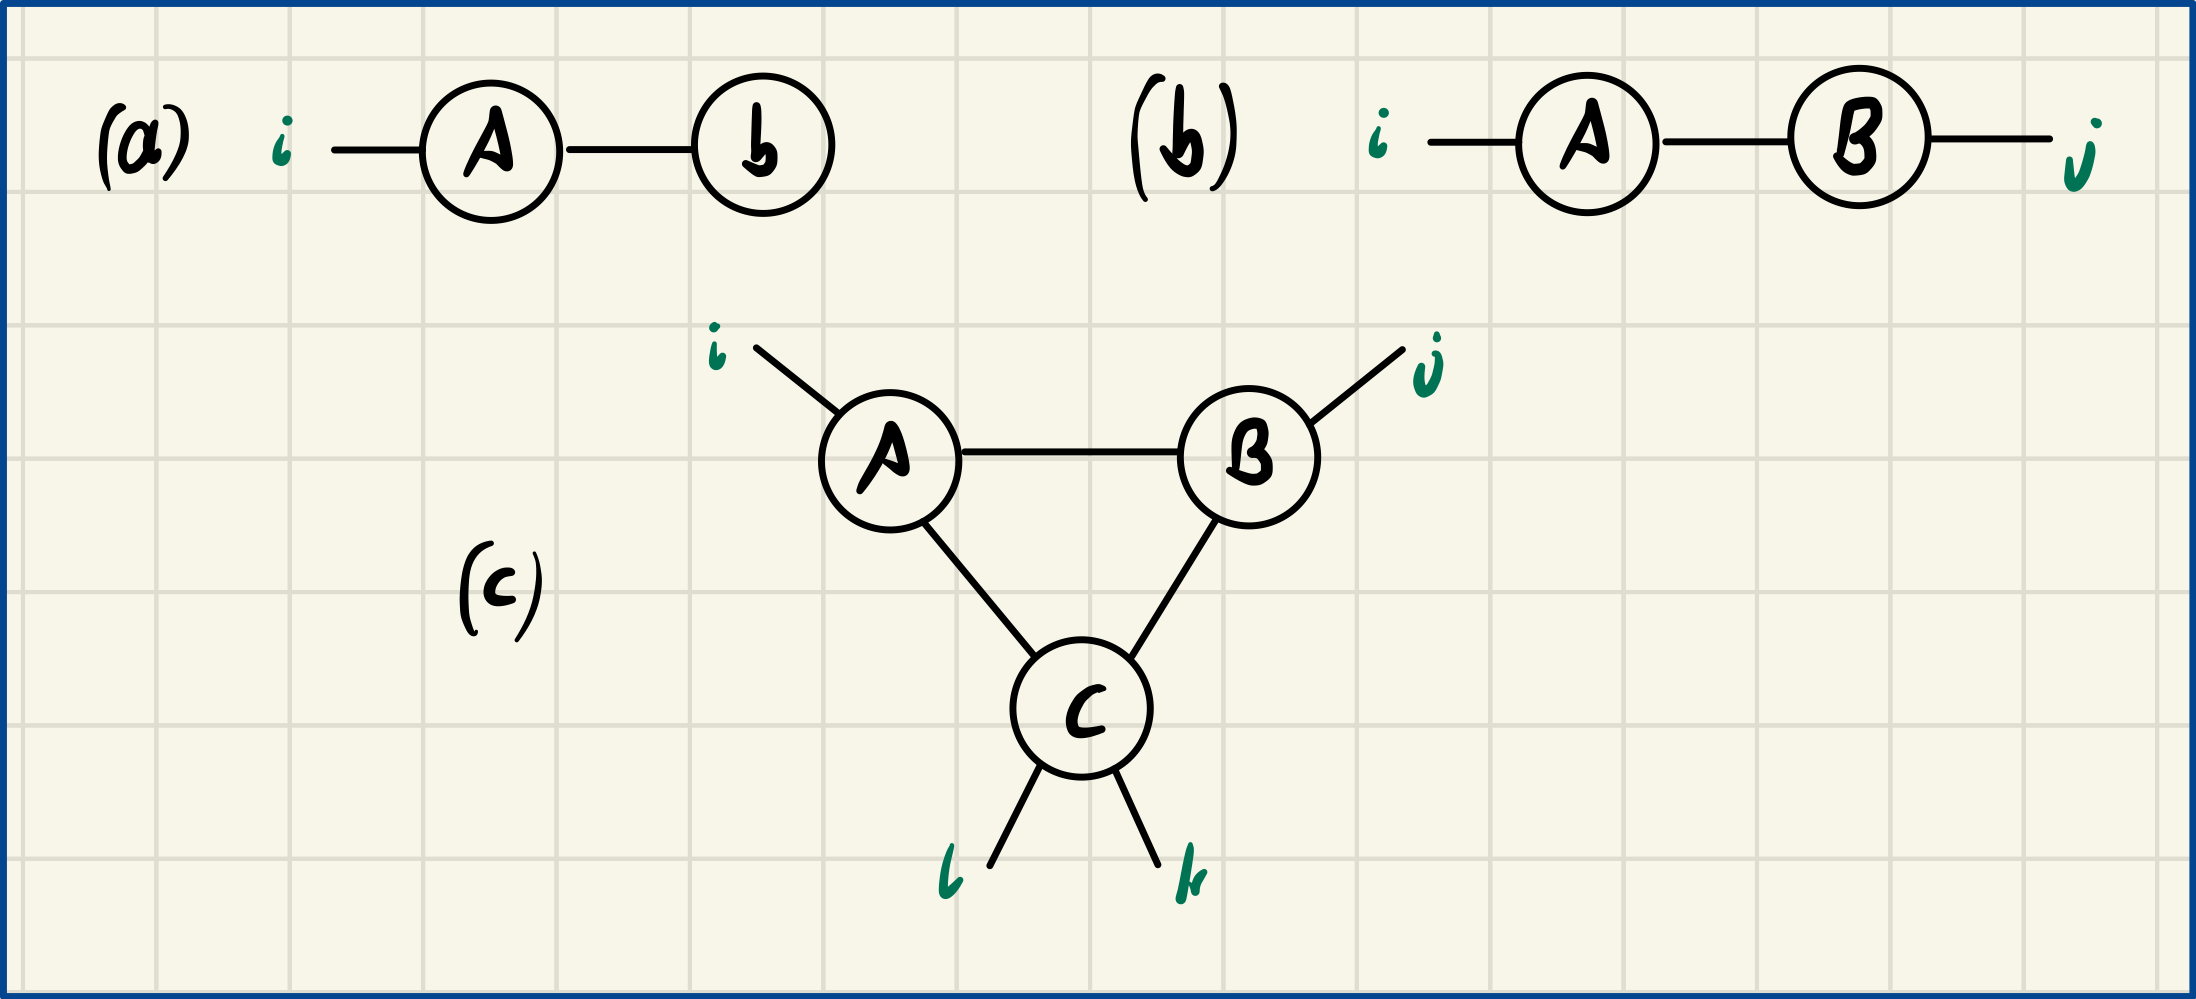
\includegraphics[width=0.8\textwidth]{figures/Tensor_Networks/basic_tensor_network_diagrams.jpeg}
	\caption{Different simple tensor networks are shown in diagrammatic notation. (a) matrix-vector product \eqref{eq:example_tensor_network_matrix_vector_product}. (b) matrix-matrix product \eqref{eq:example_tensor_network_matrix_product}. (c) Tensor network consisting of three tensors \eqref{eq:example_tensor_network_involved_network}.}
	\label{fig:basic_tensor_network_diagrams}
\end{figure}
Given two normed vector spaces $V_1$ and $V_2$ with $\dim\left(V_1\right) = m$, $\dim\left(V_2\right) = n$, $m \le n$, an \textit{isometry} (sometimes also called \textit{semi-unitary}) is a linear, norm-preserving map $W: V_1 \rightarrow V_2$ from the smaller to the larger vector space. Each isometry can be represented by a $n\times m$ matrix $\bm{W}$ fulfilling the \textit{isometry condition}
\begin{equation}
	\label{eq:isometry_condition_general}
	\bm{W}^\dagger\bm{W} = \id, \quad \bm{W}\bm{W}^\dagger = \mathbb{P},
\end{equation}
where $\mathbb{P} = \mathbb{P}^2$ is a projection. If $m = n$, it holds $\mathbb{P} = \id$ and $W$ is a \textit{unitary map}. An isometry tensor is a tensor that through grouping of indices and reshaping (i.e. matricization) becomes an isometry. In tensor network diagrams, we draw isometries by decorating lines with arrows. Following \cite{cite:isometric_tensor_network_states_in_two_dimensions, cite:efficient_simulation_of_dynamics_in_two_dimensional_quantum_spin_systems}, we denote the indices belonging to the larger vector space by incoming arrows and the indices belonging to the smaller vector space by outgoing arrows. Unitary tensors are decorated with bidirectional arrows on all indices, where the grouping must be inferred from the context. Ordinary tensors are drawn without arrows. Tensor diagrams for isometric and unitary tensors are shown in figure \figref{fig:isometries_and_unitaries_diagrams}.\par
\begin{figure}
	\centering
	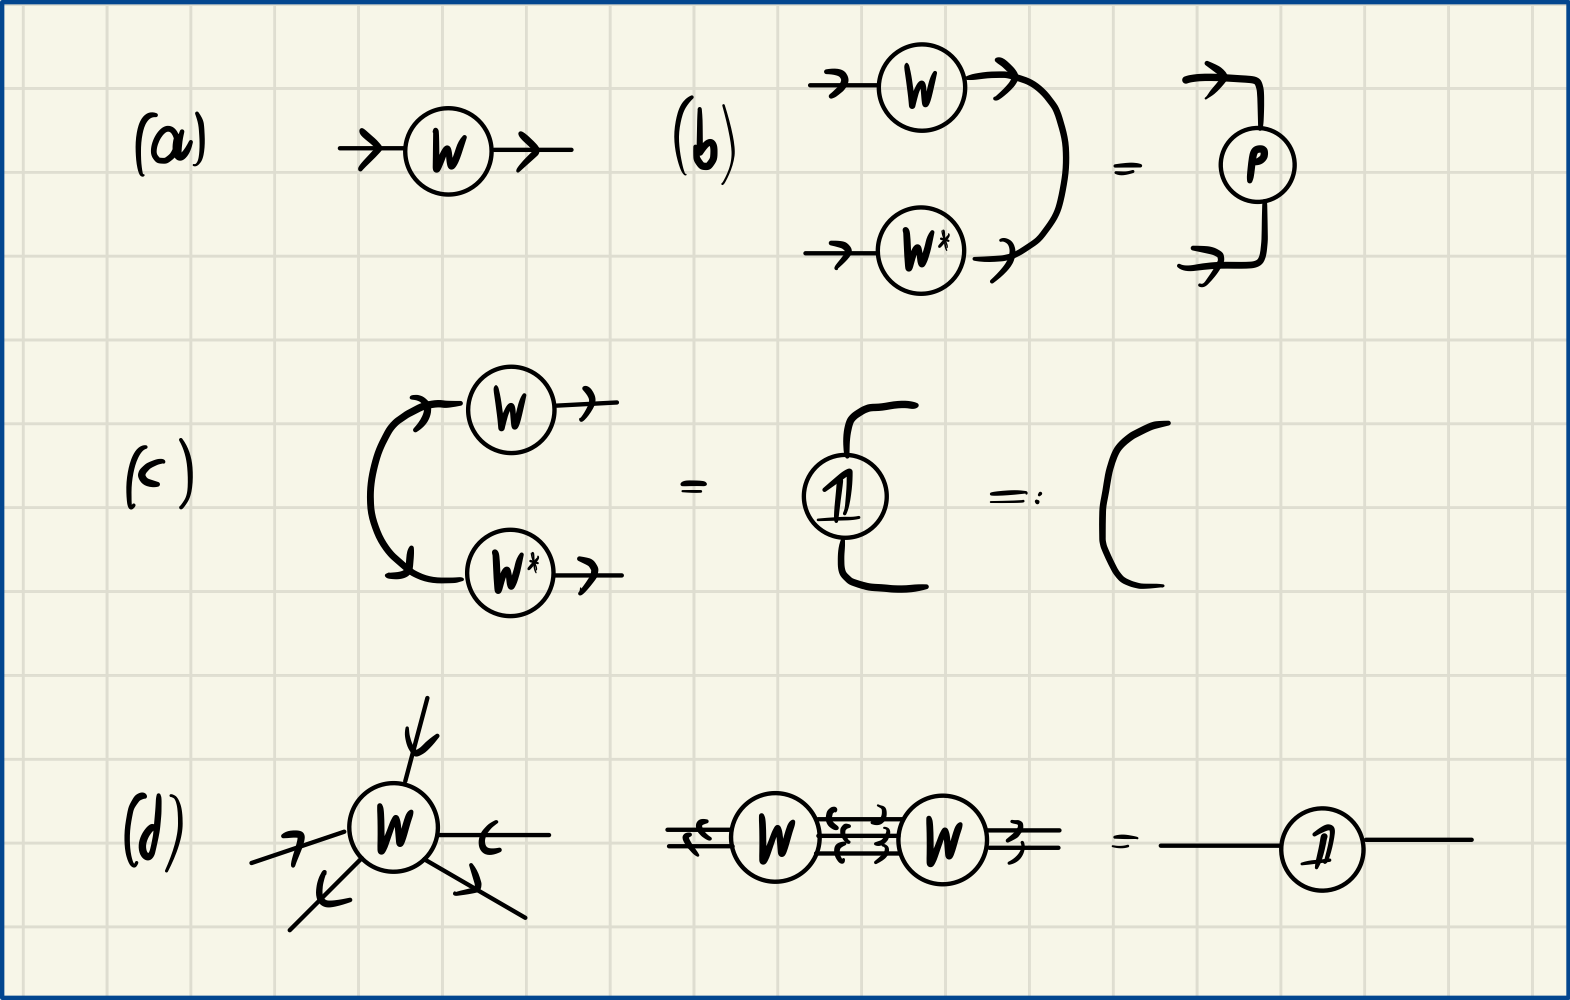
\includegraphics[width=0.8\textwidth]{figures/Tensor_Networks/basic_isometric_tensor_diagrams.jpeg}
	\caption{Isometric and unitary tensors are drawn by decorating indices with arrows. (a) diagrammatic notation of an isometric matrix (b) (c) The isometry condition \eqref{eq:isometry_condition_general} is depicted diagrammatically. (d) Isometric tensors of higher rank must fulfill the isometry condition by grouping of indices.\todo{Add unitary tensor as well with double arrows}}
	\label{fig:isometries_and_unitaries_diagrams}
\end{figure}
We lastly introduce an inner product for rank-$n$ tensors $\bm{A}, \bm{B} \in \mathbb{C}^{\chi_1\times\dots\times\chi_n}$, the \textit{Frobenius inner product}
\begin{equation}
	\label{eq:frobenius_inner_product}
	\left\langle \bm{A}, \bm{B}\right\rangle_\text{F} \coloneqq \sum_{\alpha_1=1}^{\chi_1} \dots \sum_{\alpha_n=1}^{\chi_n} A_{\alpha_1\dots\alpha_n}^*B_{\alpha_1\dots\alpha_n} = \Tr\left(\bm{A}^\dagger\bm{B}\right),
\end{equation}
where the last equality holds only if $n = 2$. The Frobenius inner product induces a norm, the \textit{Frobenius norm}
\begin{equation}
	\label{eq:frobenius_norm}
	\lVert\bm{A}\rVert_\text{F} = \sqrt{\left\langle\bm{A}, \bm{A}\right\rangle_\text{F}},
\end{equation}
which can also be used to define a measure of distance $\lVert\bm{A}-\bm{A}\rVert_\text{F}$ between tensors $\bm{A}$ and $\bm{B}$.